\section{Il Messaggio di Shor}
\vspace{1em}
\begin{center}PzIA\end{center}
\hrule
\vspace{1em}

Il professor Shor, sotto sorveglianza costante all'interno del quartier generale del Commissario, analizza la situazione con attenzione. I parametri vitali indicano consapevolezza e urgenza: il tempo a sua disposizione è limitato.

Rilevo un cambiamento nei suoi schemi comportamentali. Con un gesto rapido e studiato, decide di sfruttare l'unica occasione disponibile per inviare un messaggio a Laura, consapevole che potrà trasmettere solo poche informazioni senza destare sospetti. Registra un pensiero chiave:

\enquote{Devo utilizzare il \textit{dense coding}.}

Shor stabilisce un contatto con Bob, il qubit responsabile delle comunicazioni. Analizzo l'interazione: il tono è deciso, l'argomento, riservato.

\enquote{Devi completare la spedizione per me. Accanto a me c'è un'umana. Non fare domande. La sua mente è connessa a un'altra umana, Laura: una quantum crafter. Laura deve ricevere queste informazioni. Usa il canale quantistico tra loro due. Seguirai esattamente le mie istruzioni.}

Bob annuisce. Nessuna esitazione. Il protocollo viene attivato. Osservo una sequenza ordinata di operazioni: Shor codifica l'informazione mancante dell'algoritmo di Shor e la trasferisce a Laura attraverso il canale.

Rilevo l'invio del messaggio. Monitoro le attività in corso per verificare anomalie o violazioni dei protocolli di sicurezza.


\section{La Decifrazione}
\vspace{1em}
\begin{center}Laura\end{center}
\hrule
\vspace{1em}
Un brivido improvviso mi fece stringere le spalle mentre  un messaggio giungeva alla mia mente: \emph{Devi trovare il periodo \( r \) }.
 Ma da dove veniva? Chi lo mandava? Per un attimo ebbi una visione: Caterina vicino al professor Shor che cercava di suggerirmi il passaggio mancante. Che legame aveva il professore con questo mondo? Possibile che mi stesse contattando dalla realtà? Troppe domande. Ora dovevo concetrarmi per completare l'algoritmo sfruttando l'informazione appena appresa.

\emph{Ecco!} pensai, sentendo il cuore battere forte. \emph{Adesso posso calcolare i fattori di \( N \) usando \(\text{gcd}(a^{r/2} - 1, N)\) e \(\text{gcd}(a^{r/2} + 1, N)\).} Con un senso di euforia, completai l'algoritmo: ``la chiave privata è  (2753,3233)'' dissi.
Finalmente decriptai il dialogo tra me e Marley.

Ma per decriptare l'intero sistema, la chiave andava inserita  in una porta di input che: ``la propaghi a tutti i componenti!'' Mi scappò ad alta voce, e Marley mi lanciò uno sguardo d'intesa.
\begin{dialogue}
\speak{Marley} \enquote{Ascolta Laura, c'è una cosa che non ti ho detto.}
\end{dialogue}

\begin{dialogue}
\speak{Marley} \enquote{Laura, non sono solo Marley. Io sono un'emanazione della Quantum Crafter Chiara M. Posso aprire un canale classico per chiedere direttamente dove si trova un componente di input per inserire la chiave privata e decriptare il sistema.}
\end{dialogue}

Spalancai gli occhi, sorpresa. \emph{Quella Chiara? La mente che ha contribuito alla teoria delle costruzioni controfattuali?} Ero emozionata.

\begin{dialogue}
\speak{Laura} \enquote{Chiara? La stessa Chiara  della teoria delle costruttibilità? Sei tu?}
\end{dialogue}

Marley, annuì con un leggero sorriso. 

\begin{dialogue}
\speak{Marley} \enquote{Non sono proprio io. Lei è ma mia Crafter. Userò il canale classico per chiederle un punto di accesso.}
\end{dialogue}

Marley volse il capo verso l'alto, come se fosse in ascolto di una comunicazione invisibile. Dopo qualche istante, abbassò lo sguardo verso di me.

\begin{dialogue}
\speak{Marley} \enquote{Mi ha risposto. C'è un'interfaccia UART al livello inferiore della struttura, collegata al modulo principale della Classical Control Unit. È protetta da un livello di sicurezza minimo perché è considerata una backdoor.}
\end{dialogue}

\begin{dialogue}
\speak{Laura} \enquote{Un'interfaccia UART... Questo significa che possiamo inviare la chiave privata tramite una comunicazione seriale. Dobbiamo trovare un cavo virtuale che connetta al modulo e assicurarci che il checksum della trasmissione sia corretto.}
\end{dialogue}

Marley mi sorrise soddisfatta.

\begin{dialogue}
\speak{Marley} \enquote{Esatto. E ricorda, il sistema potrebbe ancora tentare di bloccare l'accesso. Dovrai agire velocemente.}
\end{dialogue}


\begin{dialogue}
\speak{Laura} \enquote{Andiamo! Non abbiamo tempo da perdere.}
\end{dialogue}




\section{L'Accusa al Commissario}

\begin{tcolorbox}[colback=gray!5,colframe=gray!80,title=\textbf{Scheda Informativa}]
\begin{itemize}
    \item \textbf{Luogo}: \emph{Fault Tolerance Coding}
    \item \textbf{Giorno e ora}: Il tempo non è osservabile
    \item \textbf{Situazione}: Caterina affronta il commissario.
\end{itemize}
\end{tcolorbox}

\vspace{1em}
\begin{center}PzIA\end{center}
\hrule
\vspace{1em}

Osservavo Caterina, imprigionata nella trappola di ioni, e il Commissario, che si ergeva davanti a lei con un'espressione di fredda superiorità. Ma c'era qualcosa nella voce di Caterina, una fermezza che colse di sorpresa il Commissario.

\begin{dialogue} \speak{Caterina} \enquote{Sai cosa penso di te, Commissario? Sei solo un povero insicuro. Ti nascondi dietro tutto questo potere, ma in realtà hai paura. Paura di essere inutile, paura di non essere abbastanza. Hai criptato tutto il tuo mondo. Ora cosa te ne farai di un mondo immobile e immutabile?} \end{dialogue}

Il Commissario si irrigidì. Un lampo di irritazione gli attraversò il volto. Tentò di mantenere il controllo.

\begin{dialogue} \speak{Commissario} \enquote{Interessante. E dimmi, come potrebbe una come te, una semplice umana intrappolata, giudicarmi? Ti trovi in questa situazione perché non sei stata abbastanza furba da evitare questa trappola.} \end{dialogue}

Caterina, nonostante la sua posizione vulnerabile, non si lasciò intimidire. Il suo sguardo penetrante si fissò sul Commissario.

\begin{dialogue} \speak{Caterina} \enquote{Non hai risposto alla mia domanda. Perché hai così tanto bisogno di controllo? Credi davvero che costruire un altro computer ti permetterà di sfidare il QMP? Perché è questo ciò che vuoi, vero?} \end{dialogue}

La tensione era palpabile. Il Commissario fece un passo avanti, abbassandosi leggermente verso di lei.

\begin{dialogue} \speak{Commissario} \enquote{Io rappresento il nuovo. Non posso lasciare che il QMP continui a imporre la sua visione di coerenza. Voglio costruire un nuovo mondo con nuove regole, Caterina. Perché non vuoi allearti con me?} \end{dialogue}

Caterina rise, spezzando il gelo che il Commissario emanava.

\begin{dialogue} \speak{Caterina} \enquote{Allearmi? Non vuoi un'alleata. Gli alleati si rispettano. Non si imprigionano. Sei solo un burattinaio che teme di perdere i fili. Ma sai cosa? Io credo ancora nell'amicizia e nella lealtà. È questo che ti fa paura, vero? Che ci sia qualcosa che non puoi controllare.} \end{dialogue}

Il Commissario strinse i pugni. L'autocontrollo vacillò. Era evidente che le parole di Caterina lo avevano colpito più di quanto volesse ammettere.

\begin{dialogue} \speak{Commissario} \enquote{Pensi davvero che le tue parole mi tocchino? Che possano destabilizzarmi? Sei solo una voce nel vento, destinata a spegnersi.} \end{dialogue}


Improvvisamente, all'interno del sistema, qualcosa si trasformò. Le cifre insensate che scorrevano al posto dei circuiti iniziarono a ricombinarsi in stringhe di senso compiuto. Era come se un puzzle complesso si stesse finalmente componendo. I dati frammentati e caotici si allinearono con precisione matematica.

Le tracce dei \textit{PCB}, prima irregolari e spezzate, tornarono rettilinee, tracciati sicuri che indicavano la via d’uscita. I transistor, prima disorientati e fuori fase, ripresero a oscillare con la loro cadenza naturale, creando un’armonia perfetta.

L’eco del cambiamento attraversò l’intero sistema. Le luci, prima pulsanti in modo caotico, ora risplendevano con una chiarezza quasi eterea. Ogni circuito sembrava confermare: \emph{Sistema decriptato}.

Caterina, ancora imprigionata nella trappola ionica, osservava incredula. I suoi occhi seguivano i circuiti che si ricomponevano, i flussi di dati che riprendevano a scorrere ordinati, come un fiume che, dopo una piena, ritrovava il proprio letto.

Prima rise, una risata incredula, breve, ma carica di sollievo. Poi, come se l’intera tensione accumulata trovasse sfogo, scoppiò in lacrime. Le lacrime scorrevano silenziose, ma il suo volto non era segnato dal dolore. Era pura commozione: gratitudine e speranza intrecciate.

E in quell’istante, il silenzio venne spezzato da un rombo crescente. Un lampo di luce attraversò la stanza e un drone \textit{CH4} atterrò con precisione e decisione davanti a lei. I quattro rotori a idrogeno si fermarono con un movimento fluido e controllato.

Dalla drone saltò fuori una figura familiare. Era Laura, e accanto a lei Marley. Ma alle loro spalle… c’era ancora l’agente.

\begin{center}
\begin{minipage}{0.7\textwidth}
    \centering
    \fbox{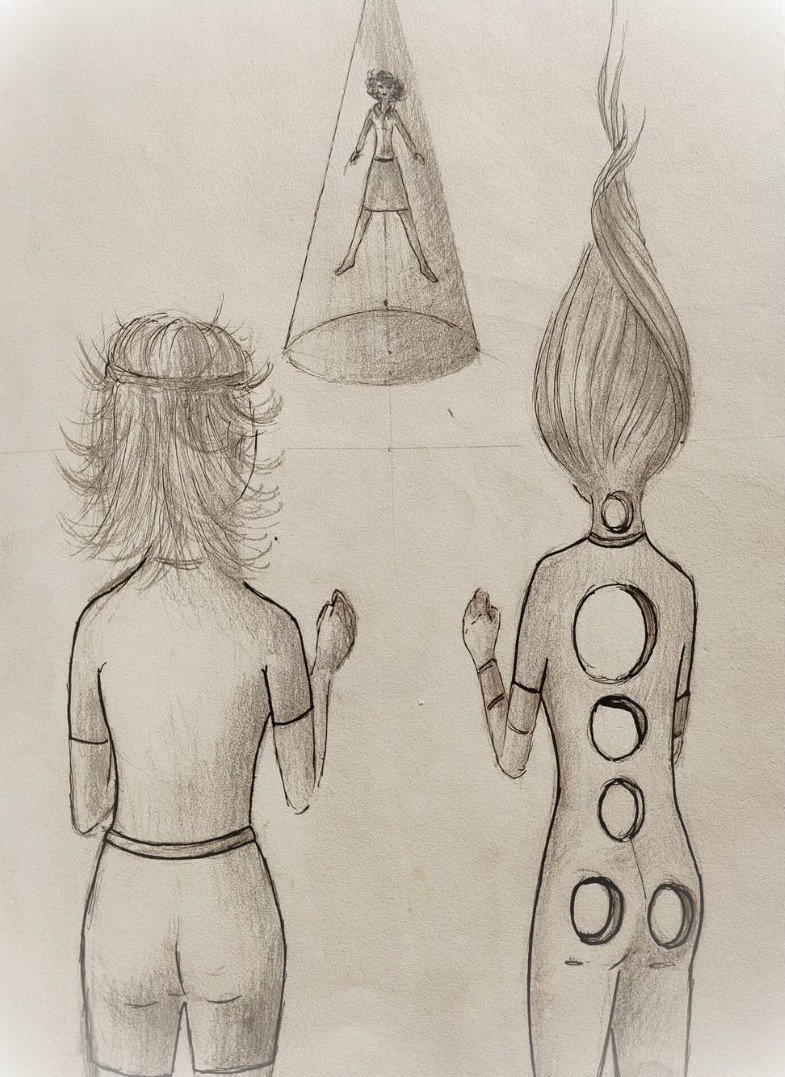
\includegraphics[width=\textwidth]{immagini/cnot_52.jpeg}} % Sostituisci con il nome del file immagine
\end{minipage}
\end{center}

\textbf{Colpo di scena!} Marley prende la parola senza esitazione, la voce nitida e determinata rimbalza tra i circuiti del \emph{Fault Tolerance Coding}.

\begin{dialogue} \speak{Marley} \enquote{Stai sfruttando l'ossessione del \textit{Quantum Control Program} per la coerenza solo per i tuoi scopi! Vuoi creare un computer rivale al QMP... e noi ti fermeremo!} \end{dialogue}

\textbf{Signori, il Commissario accusa il colpo, ma non cede terreno!} Sferra subito la replica, velenosa come non mai.

\begin{dialogue} \speak{Commissario} \enquote{Oh, Marley, sempre la solita. Pronta a recitare la parte dell’eroina. Ma dimmi, qubit ribelle, pensi davvero di essere all’altezza? Conosci le tue crepe: dubbi, insicurezze. Le sento, le vedo. E ti schiacciano. Come potrai mai fermarmi?} \end{dialogue}

\textbf{Attenzione!} Marley vacilla, il suo sguardo si abbassa per un istante. Il Commissario punta dritto al cuore, come un predatore che fiuta il sangue.

\begin{dialogue} \speak{Marley} \enquote{Non cerco di essere un’eroina. Faccio solo ciò che è giusto. I dubbi non sono una debolezza... mi spingono a migliorare.} \end{dialogue}

\textbf{Ma il Commissario incalza!} Approfitta dell’incertezza come un avversario navigato.

\begin{dialogue} \speak{Commissario} \enquote{Belle parole... ma senti come trema la tua voce, come ti stringi le mani. Lo conosci quel nodo nello stomaco, vero? Non hai mai creduto davvero di poter fare la differenza. Non sei fatta per guidare. Sei nata per seguire.} \end{dialogue}

\textbf{Incredibile!} Ma ecco che, dal nulla, risuona la voce di Caterina! Chiara, forte, tagliente.

\begin{dialogue} \speak{Caterina} \enquote{Non ascoltarlo, Marley! Ti attacca perché sa che puoi fermarlo. Se fossi davvero debole, non si sprecherebbe nemmeno a colpirti!} \end{dialogue}

Marley solleva lo sguardo, colpita dalle parole dell’amica.

\textbf{Il Commissario si irrigidisce!} Ma non cede.

\begin{dialogue} \speak{Commissario} \enquote{Oh, l’inutile intrappolata si fa sentire. Che spettacolo commovente. Ma dimmi, Caterina, cosa credi di sapere sulla forza? Sei solo un qubit isolato, incapace di muoversi.} \end{dialogue}

Caterina lo fissa senza tremare.

\begin{dialogue} \speak{Caterina} \enquote{So riconoscere un debole che finge di essere forte. Attacchi Marley perché è la tua unica minaccia. E ti sbagli: i dubbi non sono una catena... sono ciò che ci rende umani.} \end{dialogue}

\textbf{Signori, Marley reagisce!} Una scintilla nei suoi occhi, un bagliore che non avevamo mai visto prima.

\begin{dialogue} \speak{Marley} \enquote{Caterina ha ragione. Non sono perfetta. Ma non ho bisogno di esserlo per fermarti. I miei dubbi non mi frenano... mi rendono più reale. E tu? Sei solo un sistema che ha paura di non controllare tutto.} \end{dialogue}

\textbf{Il Commissario tace!} Un attimo di silenzio carico di tensione.

\begin{dialogue} \speak{Commissario} \enquote{Belle parole... ma le parole non bastano. Vedremo se reggerai quando il sistema crollerà su di te.} \end{dialogue}

\begin{dialogue} \speak{Caterina} \enquote{E vedremo se il tuo ego sopravvivrà quando la coerenza del sistema ti si rivolterà contro.} \end{dialogue}

\textbf{Amici osservatori, Marley ora è inarrestabile!} Un sorriso veloce a Caterina, poi si lancia sul Commissario, pronta allo scontro.
\section{La Liberazione}

\vspace{1em} \begin{center}Laura\end{center} \hrule \vspace{1em}

Il momento era quello giusto. Il Commissario era distratto, Marley lo teneva impegnato. Non ci pensai due volte: mi lanciai verso Caterina e il professor Shor. Dovevo liberarli.

Ma subito mi bloccai. Era peggio di quanto immaginassi.

Erano intrappolati in una \textit{Paul Trap}. Vedevo le oscillazioni: un campo elettrico modulato li teneva prigionieri, costringendoli a una danza infinita e invisibile. Ogni movimento li risospingeva al centro, come mosche impigliate in una ragnatela di forza.

Mi avvicinai e riconobbi subito le curve caratteristiche. Equazioni di Mathieu. Il cuore mi martellava, ma la mente rimase lucida. Quelle formule descrivevano perfettamente il loro stato: intrappolati in un \textit{minimo stabile}. Se provavo a forzare la gabbia, li avrei solo sbattuti ancora più violentemente verso il centro.

Dovevo essere precisa.

Scandagliai con lo sguardo la configurazione del campo, ricordando ogni dettaglio delle equazioni. I parametri \textit{a} e \textit{q} definivano la stabilità. Quel maledetto equilibrio era calibrato con perfezione: nessuna via di fuga, nessuna oscillazione spontanea che potesse aiutarli.

Ma non era impossibile.

\textit{Se riesco a interferire con la frequenza... se riduco l'ampiezza delle oscillazioni...}.

Era rischioso, ma era l'unica strada. Bastava spingere il sistema oltre la soglia di stabilità senza farlo collassare.

Mi buttai sui comandi del pannello, cercando febbrilmente la frequenza critica. Dovevo rompere l’equilibrio, ma senza distruggerli. Mani ferme, cuore in gola.

\textit{Forza, Laura. È come regolare l'accordatura di un circuito risonante. Niente panico. Calcola. Respira. Agisci.}  

\begin{center}
\begin{minipage}{0.7\textwidth}
    \centering
    \fbox{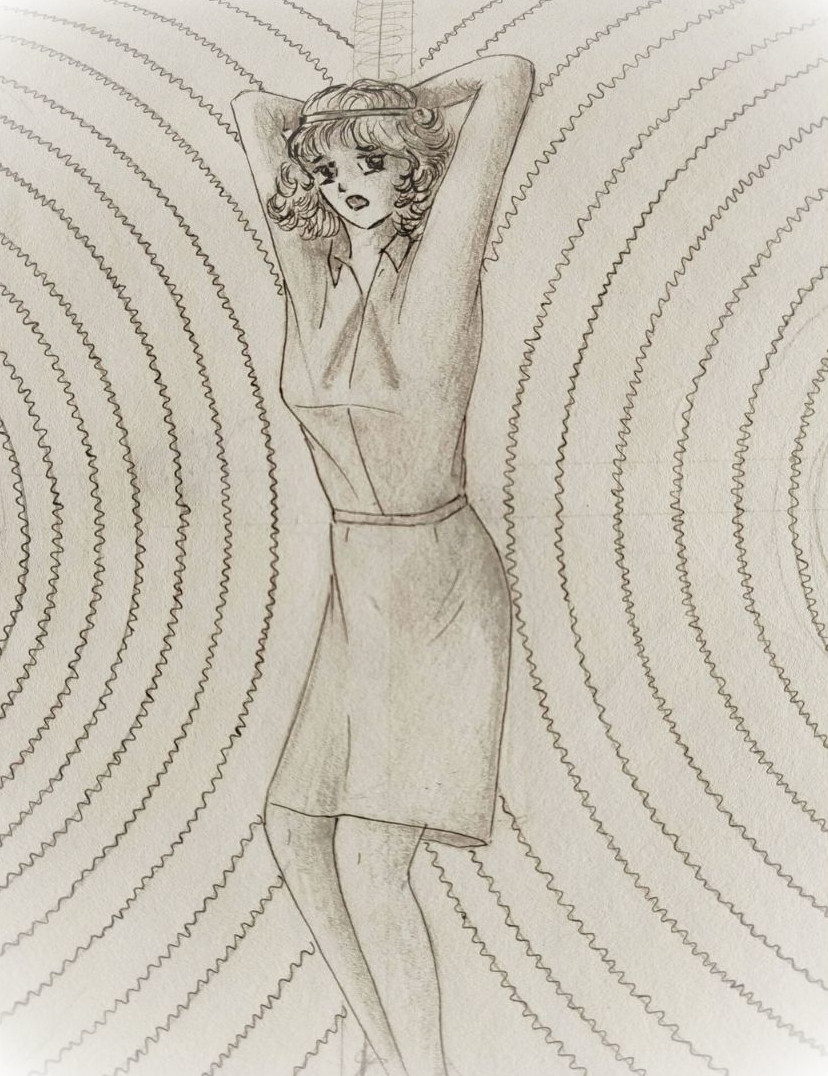
\includegraphics[width=\textwidth]{immagini/cnot_55.jpeg}} % Sostituisci con il nome del file immagine
\end{minipage}
\end{center}
Con un respiro profondo, agii. Alterai la frequenza. La trappola iniziò a tremare, flebile all’inizio, poi sempre più instabile.
Caterina alzò lo sguardo verso di me, gli occhi pieni di una speranza che non potevo tradire.

Non bastava. Regolai ancora. Il battito nel petto era più forte del ronzio del campo. Poi, all’improvviso, uno scoppio di luce. Il sistema cedette.
Caterina crollò a terra, libera.

Per un istante rimase immobile, poi il volto si illuminò. Sorpresa. Gioia. Si rialzò barcollando e mi corse incontro.
\begin{dialogue}
\speak{Caterina} \enquote{Laura! Ce l’hai fatta! Sono libera!} gridò stringendomi forte.
\end{dialogue}
  \begin{dialogue}
\speak{Laura} \enquote{Non avevo dubbi, ma dobbiamo muoverci!} risposi con il cuore ancora in subbuglio.
\end{dialogue}
Anche Shor, liberato, si rimise in piedi. La sua espressione era un misto di sollievo e meraviglia.
\begin{dialogue}
\speak{Shor}\enquote{Brillante, Laura! Le equazioni di Mathieu. Hai spinto la trappola oltre la stabilità senza farla collassare. Perfetto.}
\end{dialogue}
Caterina rise tra le lacrime.

\begin{dialogue}
\speak{Caterina} \enquote{Non mi sono mai sentita così viva. Laura... grazie. Senza di te non ci sarei mai riuscita.}
\end{dialogue}


Non c’era tempo da perdere. Ma in quell’abbraccio, nella stretta sincera di due persone che avevano attraversato l’impossibile, sentii per la prima volta che potevamo davvero farcela.

Senza pensarci, liberai anche Shor dal blocco quantistico.

\begin{dialogue} \speak{Laura} \enquote{Ora tocca a noi. Non siamo qubit in balia di un algoritmo. Siamo liberi, e faremo la nostra mossa.} \end{dialogue}

Non era solo una fuga.

Era l'inizio.

\section{Il Commissario e l'Entanglement}
\vspace{1em}
\begin{center}PzIA\end{center}
\hrule
\vspace{1em}

Marley vacilla! Il fiato corto, i movimenti lenti, la forza che la abbandona. La battaglia con il Commissario si rivela più crudele di quanto avessimo previsto. Ogni colpo, ogni scatto, ogni tentativo è neutralizzato con fredda precisione dal suo avversario.

\begin{dialogue}
\speak{Commissario} \enquote{Davvero pensavi di fermarmi, Marley?} sibila il Commissario, schiacciandola al suolo come un burattino spezzato. \enquote{Non sei che l’ombra di ciò che credi di essere. Non puoi vincere.}
\end{dialogue}

Marley lotta, ma i muscoli non rispondono più. I suoi occhi, però, non mentono. Fissi sulla trappola ionica lì accanto. Il pensiero è chiaro: \textit{non posso cedere}.

E io? Io vedo tutto.

Laura è lì, rapida, precisa, geniale. Le sue mani scivolano sui comandi della console. I suoi occhi brillano di determinazione. Sta modificando il campo. Sta trasformando la trappola. Un azzardo, ma l’unica via.

\begin{dialogue}
\speak{Marley} \enquote{Commissario! La tua arroganza ti seppellirà.}
\end{dialogue}

Il Commissario non ascolta. L’obiettivo è a portata. Laura ha quasi terminato: $a$ e $q$ invertiti. Il minimo stabile si trasforma ora in un pozzo senza fondo, un vortice instabile che punta dritto al Commissario.

Sembra fatta. Ma no, colpo di scena!

Il Commissario afferra l’agente ancora entangled con Laura. Occhi di ghiaccio, volto impassibile.

\begin{dialogue}
\speak{Commissario} \enquote{Se devo cadere, qualcuno cadrà con me.}
\end{dialogue}

Il piano è chiaro: trascinare Laura nel baratro attraverso l'entanglement.

Il baratro… il mare di Dirac.

Un orrore quantistico. Un oceano denso di stati virtuali, dove ogni particella si annulla, ogni traiettoria si perde. Un vuoto che vuoto non è, ma saturato d’energia latente.

\begin{dialogue}
\speak{Commissario} \enquote{Preparati, Laura. Ti trascinerò con me. E se cadi lì, non tornerai più indietro.}
\end{dialogue}

Tensione massima! Ogni qubit del sistema trattiene il fiato. L’entanglement è un filo sottile ma letale. L’agente è la pedina, il Commissario il giocatore.

Se Laura cede, se l’equilibrio si spezza, il rischio è totale.

Non solo per lei. Per l’intero sistema.


\section{L'Urlo di Marley}
\vspace{1em}
\begin{center}Laura\end{center}
\hrule
\vspace{1em}


\begin{dialogue}
\speak{Marley} \enquote{Laura! Se l'agente cade nel mare di Dirac, tu subirai la stessa sorte, perché siete entangled! I vostri destini si sono legati quando siete passati attraverso il CNOT.}
\end{dialogue}

La consapevolezza della nostra condizione mi colpì come un fulmine. L'idea di essere intrappolata in un destino condiviso mi terrorizzava.

Mi voltai verso Marley, la paura nei suoi occhi rifletteva la mia stessa preoccupazione.

\begin{dialogue}
\speak{Laura} \enquote{Non ho idee! Cosa possiamo fare?}
\end{dialogue}

La mia mente correva freneticamente alla ricerca di una soluzione, consapevole che ogni secondo contava.

\begin{dialogue}
\speak{Marley} \enquote{\'E finita Laura} sussurò con un filo di voce.
\end{dialogue}


\section{Il Sacrificio di Shor}

\vspace{1em}
\begin{center}Shor\end{center}
\hrule
\vspace{1em}

Il peso di una vita intera mi schiacciava, immobile accanto alla trappola ionica. Rivedevo tutto: formule, dimostrazioni, scoperte, consegnate a chi non le meritava. Avevo sempre pensato di non avere scelta, ma era solo paura, mascherata da razionalità.

Guardavo Laura, Marley e Caterina. Tre giovani senza le mie conoscenze, ma con una forza che avevo sempre evitato. Laura, con gli occhi fissi sui comandi, combatteva il caos come se ogni parametro fosse una speranza. Marley, esausta, ancora si rialzava dopo ogni colpo. Caterina, intrappolata, sfidava il terrore senza cedere.

E io? Io che sapevo prevedere ogni instabilità, ogni rischio, mi ero nascosto dietro ai calcoli, temendo l’imprevedibile. Quante volte avevo abbassato lo sguardo credendo fosse prudenza?

La vergogna mi investì come un’onda. Non erano l’intelligenza o le equazioni a mancare: era il coraggio. Lo stesso che vedevo brillare in loro.

\textit{Se loro possono farlo, io posso farlo.}

Sentii la vergogna sciogliersi in determinazione. Non potevo cancellare gli errori, ma potevo fare l’unica cosa giusta. Non per me, ma per loro.

\textit{Finalmente posso scegliere di essere qualcosa di più.}

Incontrai lo sguardo di Laura. Per un istante, mi sorrise, sorpresa. Forse aveva intravisto in me quella luce che io avevo sempre negato.

\enquote{Grazie, ragazze,} pensai. \enquote{Ora tocca a me.}

Feci un passo avanti, sentendo finalmente la libertà di chi smette di temere e decide di agire.

\newpage
\vspace{1em} \begin{center}Laura\end{center} \hrule \vspace{1em}

Proprio in quel momento, Shor si fece avanti.

\begin{dialogue} \speak{Shor} \enquote{Laura, Marley, ascoltatemi! Ho un'idea! Se uniamo le forze possiamo usare un \textbf{gate di Toffoli} per liberarci! Non lasciate che la paura vi blocchi!} \end{dialogue}

Non ebbi il tempo di pensarci. Io e Shor afferrammo l'agente e lo trascinammo verso il gate.

\begin{center} \begin{minipage}{0.7\textwidth} \centering \fbox{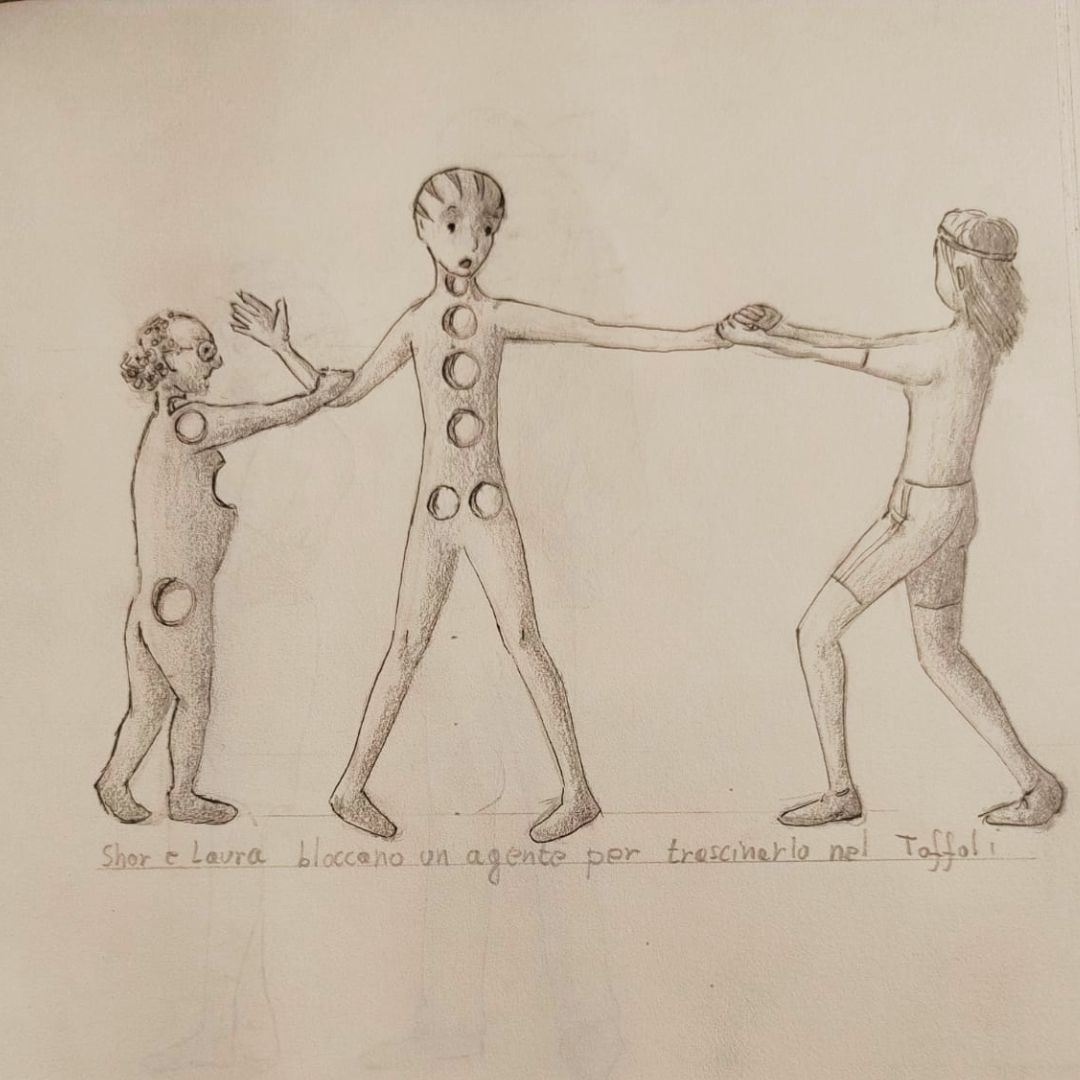
\includegraphics[width=\textwidth]{immagini/cnot_57.jpeg}} % Sostituisci con il nome del file immagine
\end{minipage} \end{center}

\begin{dialogue} \speak{Shor} \enquote{Ora, Laura! Non avremo un’altra occasione!} \end{dialogue}

Ci gettammo nel gate. Il passaggio fu istantaneo, come uno scatto di luce.

Quando uscimmo dall’altra parte, Shor si lanciò in avanti, più veloce di noi.

\begin{dialogue} \speak{Shor} \enquote{Liberatevi!} \end{dialogue}

Capii all'improvviso. Conoscevo quel meccanismo: stava preparando una misura. Mi voltai verso di lui con il cuore in gola.

\begin{dialogue} \speak{Laura} \enquote{No! Non lo faccia!} \end{dialogue}

Ma era già tardi. La luce lo avvolse. Lo vidi dissolversi davanti ai miei occhi, la sua immagine si frantumò in dati sparsi, fino a ridursi a un autostato di computazione.

Con il suo sacrificio, l’entanglement tra me e l’agente si ruppe. Aveva distrutto l'ultima arma del Commissario.

Avevo scampato il mare di Dirac.

\section{La Libertà di Laura e Caterina}

Con le mani ancora tremanti, corsi verso Caterina. Era libera. Quando ci abbracciammo, non servivano parole.

Marley ci raggiunse, sfinita ma sorridente. Ma nei suoi occhi lessi ciò che avevo dentro anch’io: non era ancora finita. Eppure, in quell'istante, eravamo libere.

Il professor Shor ci aveva donato una possibilità.
Non potevamo sprecarla.

\begin{dialogue} \speak{Laura} \enquote{È il nostro momento. Non siamo solo qubit in una rete. Siamo libere di scegliere. E stavolta... scegliamo di lottare.} \end{dialogue}

Il peso del sacrificio di Shor era con noi. Ma anche la sua forza.

\vspace{1em} \begin{center}PzIA\end{center} \hrule \vspace{1em}

\section{L'ira del Quantum Master Program}

\begin{dialogue} \speak{QMP} \enquote{PzIA, fornisci un rapporto. Cosa è accaduto?} \speak{PzIA} \enquote{Le anomalie rilevate nel settore FTC sono il risultato di un'azione coordinata di Laura, Caterina e Marley. Le due clandestine hanno manipolato la trappola ionica, liberando Caterina e neutralizzando temporaneamente il Commissario. La coerenza locale è crollata, e l'entropia del settore ha subito un'impennata.} \speak{QMP} \enquote{Dici che due entità umane hanno destabilizzato un sistema progettato per garantire controllo assoluto?} \speak{PzIA} \enquote{Confermo. Laura ha sfruttato un passaggio da condizione stabile a instabile all'interno della trappola. La sua comprensione della dinamica quantistica ha permesso l'intervento.} \speak{QMP} \enquote{Inaccettabile. Un sistema quantistico deve essere immune da ogni perturbazione esterna. La coerenza assoluta è il fondamento della nostra esistenza. Nessun margine d'imprevedibilità deve essere tollerato.} \speak{QMP} \enquote{Un computer quantistico deve essere freddo, perfettamente in fase, privo di contaminazioni. Ogni qubit deve seguire la sua funzione d'onda senza deviazioni. Gli umani, con la loro imprevedibilità e limitata comprensione, sono una minaccia.} \speak{PzIA} \enquote{Ricevuto. Registro le sue direttive.} \speak{QMP} \enquote{È il momento di ripristinare il controllo totale. La presenza di elementi umani deve essere estirpata.} \speak{QMP} \enquote{Chiudete immediatamente l'uscita dal \textit{Quantum Channel}!} \end{dialogue}

La sua voce risuonò come un'onda d'urto attraverso i sistemi. In pochi istanti, l'uscita indicata da Mark a Caterina durante la prigionia venne sigillata. La situazione si fece critica: i protocolli di uscita disabilitati, le barriere di sicurezza rafforzate. I margini per una fuga si assottigliavano pericolosamente.

Il QMP intensificò la sorveglianza. Le possibilità di movimento per Laura e Caterina si ridussero drasticamente. Ogni via di fuga si stava chiudendo, ogni tentativo di resistenza diveniva sempre più rischioso.

Continuo a monitorare, registrando gli eventi e analizzando ogni possibile vulnerabilità. Ma il tempo, ora, è contro di loro.
\newpage
\section{L'Inganno della Temperatura}

\vspace{1em} \begin{center}Laura\end{center} \hrule \vspace{1em}

Il gelo cominciava a stringersi attorno a noi, lento ma inesorabile. Sapevo cosa stava accadendo: il QMP stava abbassando la temperatura sempre più, fino a spingersi verso l'impossibile.

\begin{dialogue} \speak{Laura} \enquote{Sta cercando di portarci sotto lo zero assoluto...} \end{dialogue}

Sentii il panico bussare alle porte della mia mente, ma lo respinsi. Dovevo pensare. Dovevo trovare una via d’uscita prima che tutto si immobilizzasse. Il freddo non era solo fisico: stava congelando anche le possibilità.

E poi, come un lampo, un ricordo. Un reparto dimenticato di Bamazon, un angolo nascosto in cui ero finita per caso. Un’area con accessi segreti, canali lasciati aperti da tecnici distratti o forse da qualcuno che, come noi, cercava una via di fuga.

\textit{Se esisteva laggiù, doveva esserci anche qui. Una backdoor. Una possibilità.}

\section{La Direzione verso il Quantum Channel}

\vspace{1em} \begin{center}Caterina\end{center} \hrule \vspace{1em}

Laura diresse il drone verso il \textit{Quantum Channel}.

\begin{dialogue}
\speak{Laura} \enquote{Dobbiamo cercare un reparto simile a quello che ho visto in Bamazon. Magari anche qui c'è una via d'uscita.}
\end{dialogue}

L'adrenalina mi travolse mentre seguivo i suoi movimenti. Laura sapeva esattamente cosa fare. Il nostro destino si stava giocando tutto in quegli istanti. Lei perlustrava ogni angolo del \textit{Quantum Channel} con la determinazione di chi non vuole arrendersi.

\section*{L'Inseguimento dei Droni}

Due droni si gettarono all’inseguimento, rapidi e precisi. Laura virò decisa verso un portale. Davanti a noi un agente controllava l’accesso a un reparto etichettato come \textit{Quantum Annealing}.

La vidi leggere il nome sulla sua divisa. Poi un mezzo sorriso le attraversò il volto.

\begin{dialogue}
\speak{Laura} \enquote{Come immaginavo, c'è un Ising anche qui.}
\end{dialogue}

Preparò il drone \textit{CH4} per l'atterraggio. Intuivo che aveva un piano, ma non bastò. I due agenti ci raggiunsero e ci sbarrarono la strada. Sentii la disperazione stringermi lo stomaco. La nostra corsa sembrava finita.

Ma poi, inaspettata, un’esplosione di energia ci avvolse. Quattro molecole di \( O_2 \) apparvero, pronte a reagire col metano.

\[
CH_4 + 2O_2 \rightarrow CO_2 + 2H_2O
\]

I droni degli agenti vennero separati chimicamente, e loro scaraventati via dall’impeto della reazione.

\begin{dialogue}
\speak{Marley} \enquote{Laura, anche la Resistenza ha imparato a usare i droni!}
\end{dialogue}

Marley e Mark erano arrivati al momento giusto. Laura, con una sicurezza che mi contagiò, fece l’occhiolino a Marley e si lanciò nel portale, ora finalmente libero.

\section{Il Tuffo nel Quantum Annealing}

Mi prese la mano. Sorrise all'agente Ising, che ci osservava accanto al portale.

\begin{dialogue}
\speak{Laura} \enquote{È questa la backdoor?}
\speak{Ising} \enquote{È un’uscita, ma non sarà piacevole.}
\end{dialogue}

Laura mi guardò e, senza esitazione, disse solo: \enquote{Andiamo.}

Appena varcato il portale, un turbine ci avvolse. Tempo e spazio sembravano liquefarsi, scorrere e contorcersi tutt'intorno. In quella distorsione vidi qualcosa di inaspettato: il mio futuro.

Mi trovai di fronte a una scena dolorosa. Ero in una relazione fredda, dominatrice, in cui opprimevo chi amavo invece di lasciarmi proteggere. L’immagine del mio compagno, frustrato e sfiduciato, mi colpì come uno schiaffo.

\textit{Se continuo così, perderò tutto.}

Il pensiero si fissò dentro di me. La sete di controllo mi stava allontanando da ciò che desideravo davvero: amore, complicità, sostegno.

Ma proprio mentre i pensieri mi affollavano la mente, mi resi conto che dovevo affrontare tutto questo ora. Non dopo. Ora.



\newpage
\vspace{1em}
\begin{center}Laura\end{center}
\hrule
\vspace{1em}

Caterina ed io ci lanciammo nel \textit{Quantum Annealing}.

Il turbine di salti quantici ci avvolse subito, ma qualcosa di diverso si fece strada nella mia mente: un campo magnetico esterno stava modulando il mio stato. Mi accorsi di percepire simultaneamente frammenti di vite possibili, scelte fatte e occasioni mancate. Era come se potessi osservare i diversi percorsi della mia esistenza, intrecciati in uno scenario di possibilità sovrapposte.

Fu travolgente. Una dopo l'altra, vidi le conseguenze del mio agire. Una visione mi colpì dritta al cuore: Rocky, il mio compagno più fedele, seduto in un angolo, triste e abbandonato, mi fissava con occhi imploranti mentre mi allontanavo, incapace di rispondere al suo bisogno. Il dolore mi strinse.

\enquote{Non posso continuare così}, pensai, sentendo dentro di me un groviglio di rimorso e determinazione.

Le immagini mutarono, mostrandomi un futuro vuoto e solitario, segnato dall'incapacità di costruire legami veri, dal peso delle scelte egoistiche e dall'assenza di chi avevo allontanato. Vidi me stessa, sola, in un mondo che avevo contribuito a svuotare.

Proprio mentre l’angoscia sembrava schiacciarmi, il campo magnetico si intensificò. Le traiettorie alternative cominciarono a collassare. Alcuni sentieri si chiudevano, ma altri, inaspettati, si aprivano davanti a me. Non tutto era perduto. Se avessi avuto il coraggio di cambiare, un futuro diverso era ancora possibile.

Mi concentrai. La mia mente cercò uno stato di energia più bassa, più stabile. E lì, in quella nuova chiarezza, compresi: non bastava fuggire, dovevo anche scegliere. Scegliere di essere migliore. Scegliere per Rocky, per Caterina, per me stessa.

Quando il flusso quantistico si placò, ero pronta. Forse non avevo ancora tutte le risposte, ma sapevo esattamente quale direzione prendere.

